\documentclass[journal,a4paper,twoside]{sty/IEEEtran}

%% Based on bare_jrnl.tex V1.3 2007/01/11 by Michael Shell (requires IEEEtran.cls version 1.7 or later) 

\usepackage[utf8]{inputenc}
\usepackage[slovene]{babel}
\usepackage{sty/EVrevija}

% *** GRAPHICS RELATED PACKAGES ***
\ifCLASSINFOpdf
\usepackage[pdftex]{graphicx}
\usepackage{amsfonts}           %doda zbirko matematičnih znakov
\usepackage{graphicx}           %prikz slik  
\usepackage{longtable}          %paket za tabele, ki se raztezajo čez več strani
\usepackage{float}
\usepackage{caption}
\usepackage{color}
\usepackage{mathtools}
\usepackage{amsmath}
\usepackage{media9}
\usepackage{enumerate}
\usepackage[official]{eurosym}
\usepackage{algorithm}
\usepackage[noend]{algpseudocode}
\else % or other class option (dvipsone, dvipdf, if not using dvips).
   \usepackage[dvips]{graphicx}
\fi
%\usepackage{epsfig}
\usepackage{epstopdf} % A.T. include eps images in pdftex (Miktex2.8 or higher)

% Include all other packages here
\usepackage{textcomp} % need for \textmu
%\usepackage{eurosym} %  symbol \euro
%\usepackage[cmex10]{amsmath} % *** MATH PACKAGES ***

% correct bad hyphenation here
%\hyphenation{op-tical net-works semi-conduc-tor}

\begin{document}

% naslov prispevka, lahko uporabite en linebreak \\
\title{Optimizacija digitalnih gradnikov na nivoju tranzistorjev}

\authors{Janez Puhan, Iztok Fajfar, Tadej Tuma, \'{A}rp\'{a}d B\H{u}rmen} % use ^1, ^2 for author(s) from different institutions

\address{Univerza v Ljubljani, Fakulteta za elektrotehniko, Tržaška 25, 1000 Ljubljana, Slovenija\\
E-pošta: janez.puhan@fe.uni-lj.si}

\abstract{Izdelovalci integriranih vezij za svoje procese podajajo knjižnice osnovnih digitalnih gradnikov, ki se uporabljajo pri načrtovanju digitalnih integriranih vezij. Izvedbe posameznih gradnikov na tranzistorskem nivoju so s tem določene in se med načrtovanjem vezja ne spreminjajo več. Gradniki, kot npr. medpomnilniki, logična vrata, seštevalniki, flip-flopi itd., se uporabljajo brez sprememb, kjerkoli jih načrtovalec potrebuje. Zaradi tega posamezen gradnik ni povsem prilagojen na specifično okolje v vezju, kjer se nahaja. To odpira prostor optimizaciji gradnika točno na zahteve v katerih deluje. članek opisuje primer optimizacije digitalnega gradnika na tranzistorskem nivoju. Zaradi šumnosti kriterijske funkcije je bila uporabljena robustna globalna optimizacijska metoda. Rezultati pokažejo znatno izboljšanje želenih lastnosti glede na splošni gradnik izdelovalca integriranih vezij.}

\keywords{načrtovanje digitalnih integriranih vezij, splošni osnovni gradniki, sinteza digitalnih vezij, optimizacija na tranzistorskem nivoju}

\received{19. oktober, 2010} % datum sprejema članka, lahko pustite prazno
\review{4. februar, 2011}    % datum odobritve članka, pustite prazno

% Priimki avtorjev in kratek naslov članka za tekočo glavo
\markboth{Puhan, Fajfar, Tuma, B\H{u}rmen}{Optimizacija digitalnih gradnikov na nivoju tranzistorjev}

% make the title area
\maketitle




\section{Uvod}

V nalogi je obravnavan postopek 3D rekonstukcije objektov na podlagi večih zajetih slik. Za rekonstrukcijo je uporabljena DLT (angl. \textit{Direct linear transform}) metoda. Temelji na rekonstrukciji 3D oblika iz slik, ki so zajete pri znanih kotih zasuka objekta. Pri postopku rekonstrukcije ima zelo veliko vlogo sistem s katerim zajemamo sliko. Bolje kot je zastavljen, bolj konstrastne slike dobimo. Dobro zajete slike nam olajšajo delo pri kasnejši obdelavi.



\section{Teoretično ozadje}
kalibracija in fbp algoritem (pseudo ali flowchart), poravnava

\section{Zajem slik}
Sistem s katerim smo izvajali rekonstrukcijo je blokovno prikazan na sliki ~\ref{fig:blokovna}. Objekt, ki ga želimo skonstruirati postavimo na vrtljivo pozicionirno mizo. Iz zgornje strani navzdol svetimo s homogeno, difuzno osvetlitvijo. Objekta direktno ne osvetljujemo, saj je namen osvetlitve predvsem osvetlitev ozadja z enakomerno intenziteto. Cilj je doseči čimvečjo razliko v intenziteti med opazovanim objektom in zaslonom. Za ta namen je med objekt in svetilko postavljena svetlobna ovira. Slike smo zajemali z Raspberry Pi kamero v osi na objekt in na osvetljeno ozadje. Pred kamero je dodan filter za namen filtriranja okoliške svetlobe.

\begin{figure}[H]
	\centerline{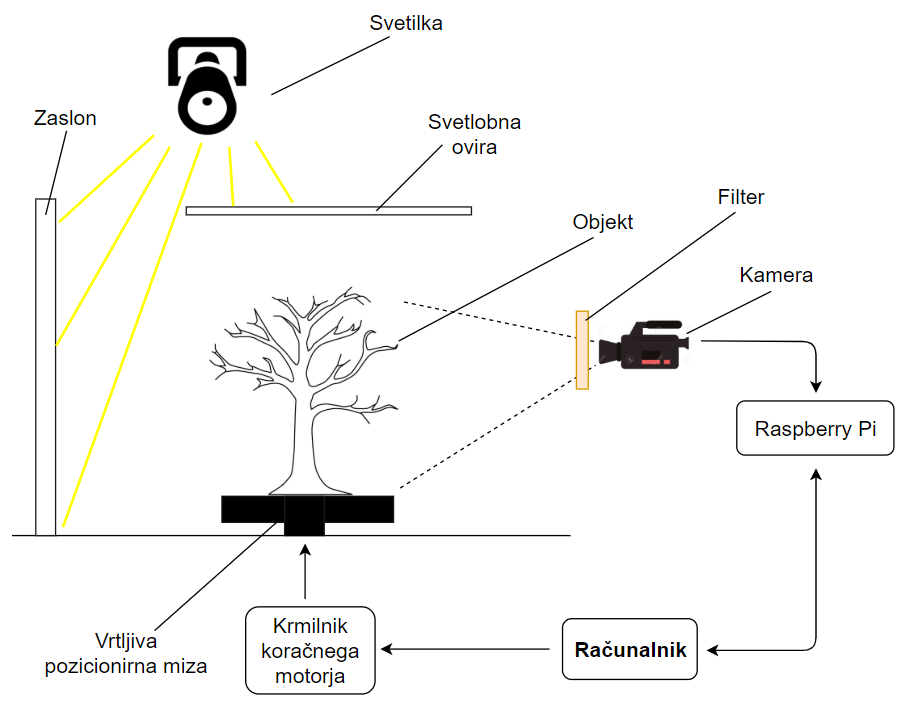
\includegraphics[width=8.2cm]{fig/blokovna_sistem}}
	\caption{Semioperacijska shema sistema.}
	\label{fig:blokovna}
\end{figure}
%
 Celoten proces zajemanja krmilnimo z računalnikom. Ta je žično povezan na krmilnik s katerim upravljamo rotirajočo pozicionirno mizo. Prav tako je računalnik brezžično povezan na Raspberry Pi. Ta zajete slike pošilja na računalnik. Objekt rekonstruiramo tako, da ga postavimo na predvideno mesto. Nato lahko pričnemo z zajemom slik. Najprej inicializiramo kamero na začetne vrednosti. Nastavimo ISO na 200, svetlost na 45 in resolucijo na 900x1000.  Objekt obračamo po začrtanih zasukih. Po vsakem izvedenem zasuku posnamemo eno sliko, ki se nato brezžično prenese iz Raspberry Pi-ja na računalnik. Postopek ponavljamo dokler objekta ne poslikamo v rangu celotnega kroga. Zajete slike ob znanih kotih zasuka se kasneje uporabijo za 3d rekonstrukcijo. V tabeli ~\ref{tab:komponente} so zapisane vse glavne komponente, ki so zajete v postavljenem sistemu. Manjše komponente kot so vijaki in nosilci v tabeli niso zajeti.

\begin{center}
	\centering
	\captionsetup{singlelinecheck = false, justification=justified}
	\captionof{table}{Komponente sistema.} 
	\label{tab:komponente} 
\begin{tabular}{|c|c|}
	\hline
	\textbf{Komponenta} & \textbf{Podrobnosti}                            \\ \hline
	Raspberry Pi        & Raspberry Pi 3 Model B                          \\ \hline
	Svetilka            & Halogenska svetilka (12V)            \\ \hline
	Zaslon              & Bela ravna plošča                               \\ \hline
	Krmilnik            & Fischertechnik stage control                \\ \hline
	Kamera              & RP Cam V2-8 MP,1080p \\ \hline
	Svetlobni filter    & Ozkopasovni filter         \\ \hline
	Svetlobna ovira     & Kartonasta zavesa                \\ \hline
		Pozicionirna miza   & Fischertechnik rotary stage                     \\ \hline
\end{tabular}
\end{center}
Primer zajete slike obravnavanega objekta je prikazan na sliki ~\ref{fig:zajeta_slika}. S slike lahko vidimo dober kontrast objekta in precejšnjo razliko v barvi in svetlosti objekta proti ozadju. 

\begin{figure}[H]
	\centerline{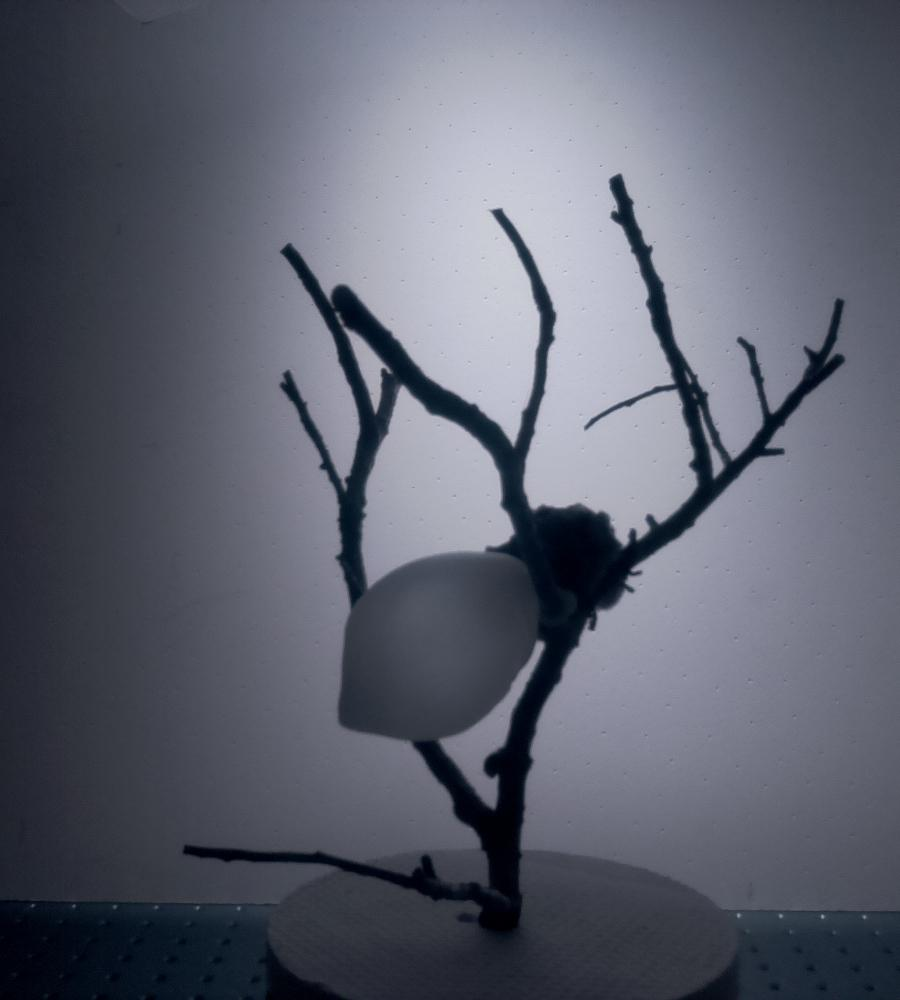
\includegraphics[width=5.2cm]{fig/zajeta_slika}}
	\caption{Zajeta slika.}
	\label{fig:zajeta_slika}
\end{figure}

\section{Rezultati}



\subsection{Vpliv kompleksnosti in kontrasta}
-  primerjava kompleksnosti modela
-  Primerjaj slab in dober kontrast slike (primer slusalk na 30 slikah)

\subsection{Število zajetih slik}
-	Ali res boljša z 90 proti 30 slikami (drevešček)


\subsection{Poravnava oblakov točk}
Za dodaten eksperiment smo izvedli medsebojno poravnavo oblakov točk. Referenčni oblak točk smo zajeli z 90 slikami in si zapolnili referenčno lego objekta na pozicionirni mizi. Nato smo izvedli še šest zajemov po 30 slik. Ob vsakem zajemu smo skeniran objekt zasukali za predpisan kot glede na referenčno lego. Tako smo zajeli oblake točk zasukane za 45, 90, 135, 18, 225 in 315 stopinj. Na sliki sta zaradi preglednosti prikazana le referenčni in zasukan oblak. Na levi strani sta oblaka prikazana pred poravnavo in na desni po poravnavi. 

\begin{figure}[H]
	\centerline{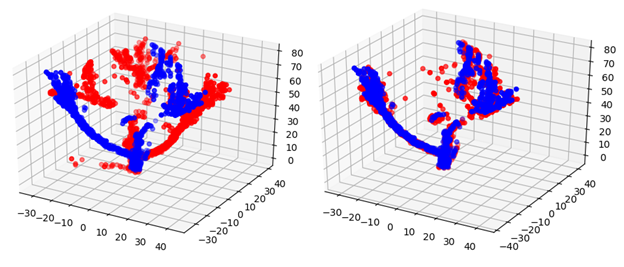
\includegraphics[width=8cm]{fig/poravnava}}
	\caption{a) neporavnana, b) poravnana.}
	\label{fig:poravnava}
\end{figure}

Po vsaki izvedeni poravnavi smo iz transformacijske matrike izsluščili kot..

 Na sliki ~\ref{fig:poravnava_graf} so z rdečo prikazani referenčni koti, z modro pa dejanski koti, ki jih dobimo s pomočjo poravnave. 

\begin{figure}[H]
	\centerline{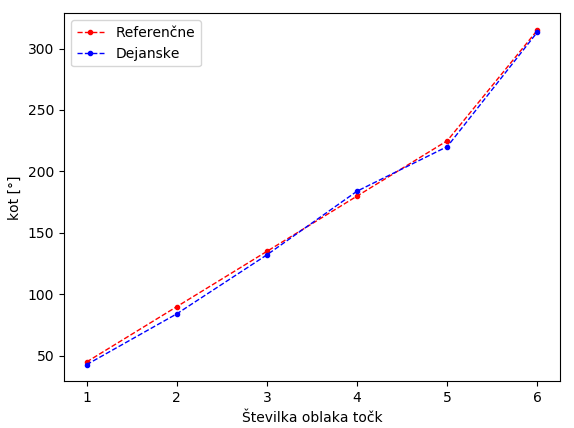
\includegraphics[width=8cm]{fig/graf_poravnave}}
	\caption{Razlika med referenčnimi in dejanskimi koti.}
	\label{fig:poravnava_graf}
\end{figure}

\subsection{Vzvratno inženirstvo}
-  mesh v blenderju in 3d print (reverse engineering)





\newpage
Pri načrtovanju digitalnega vezja načrtovalci uporabljajo osnovne gradnike ali bloke \cite{kaeslin} kot so medpomnilniki, logična vrata, seštevalniki, zatiči, flip-flopi itd. Knjižnico z digitalnimi gradniki za vsak proces izdelave integriranih vezij priskrbi izdelovalec integriranih vezij. Navadno je podanih več različic posameznega gradnika, skupaj z opisom karakteristik posamezne različice. Med postopkom načrtovanja digitalnega integriranega vezja načrtovalec simulacij \cite{hspice, kunderth, virtuoso, tuma} na tranzistorskem nivoju ne izvaja. Za izračun odziva vezja se uporabljajo opisi gradnikov na višjem nivoju \cite{thomas, pedroni}.

Posamezne različice nekega gradnika imajo v večini primerov enako topologijo. Razlikujejo se le v dimenzijah tranzistorjev, navadno v širinah in dolžinah kanalov. So rezultat prilagoditve gradnika na različne pogoje delovanja. V članku je opisana optimizacija gradnika iz knjižnice izdelovalca integriranih vezij. Zanima nas, ali je možno s pomočjo optimizacijskega postopka iz standardnega gradnika iztisniti še boljše lastnosti. S tem bi dobili tudi odgovor na vprašanje, ali je optimmizacija gradnikov na tranzistorskem nivoju smiselna, oziroma ali bi kazalo v prihodnosti z avtomatizacijo optimizacijskega postopka gradnikov na tranzistorskem nivoju generirati poljubne gradnike prilagojene na točno določene razmere v vezju.

Proces načrtovanja digitalnega vezja ASIC (Application Specific Integrated Circuit) se začne z opisom specifikacij vezja na nivoju RTL (Register Transfer Level). Nato načrtovalec vezje opisano z opisnim jezikom HDL (Hardware Description Language) simulira in popravlja, dokler odziv vezja ni zadovoljiv glede na podane zahteve. Končen opis vezja v jeziku HDL se reducira na logični nivo. Vezje na logičnem nivoju se na nivoju osnovnih gradnikov optimizira, dokler ustreznost vezja glede na zahteve v časovnem prostoru ni dosežena. Redukcijo na logični nivo in optimizacijo na nivoju gradnikov imenujemo sinteza. Sintezo načrtovalec izvede s pomočjo sintezacijskega orodja, ki pri tem izbira med osnovnimi gradniki iz knjižnice proizvajalca integriranih vezij. Delovanje končnega vezja načrtovalec preveri pred in po razporeditvi (ang. layout) tranzistorjev na rezini. V kolikor med preverjanjem ugotovi napake, ali nezadovoljivo delovanje vezja, mora proces sinteze ponoviti s strožjimi zahtevami.

Idejo uvedbe optimizacijskega postopka na nivoju tranzistorjev v tok sinteze vezja prikazuje slika \ref{synthesis_step}. Rezultat sinteze A je opis vezja na nivoju osnovnih gradnikov skupaj s časovnimi zahtevami za posamezen gradnik. Iz knjižnice so izbrane ustrezne različice posameznih gradnikov. Sledi predlagana optimizacija na nivoju tranzistorjev. Optimizacija s spreminjanjem velikosti tranzistorjev prilagodi posamezen gradnik točno na njegove časovne zahteve. Nekateri izmed izbranih gradnikov v koraku A komaj zadovoljujejo podane časovne zahteve, medtem ko imajo drugi veliko rezerve. Gradnike, ki komaj izpolnjujejo postavljene zahteve, bi lahko optimizirali na hitrost, gradnike z rezervo pa na porabo, brez da bi pri tem poslabšali lastnosti vezja. Rezultat optimizacije na nivoju tranzistorjev so razmeram prilagojeni gradniki, iz katerih bi lahko sestavili novo knjižnico. Sinteza B bi prvotno knjižnico gradnikov zamenjala s prilagojeno. Uspešna sinteza B bi tudi potrdila pravilno delovanje vezja zgrajenega iz prilagojenih gradnikov.

\begin{figure}[htb]
\centerline{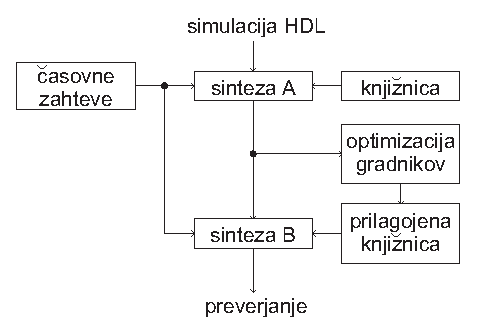
\includegraphics[width=6.5cm]{fig/synthesis_step_slo}}
\caption{Uvedba optimizacijskega postopka na nivoju tranzistorjev v tok sinteze}
\label{synthesis_step}
\end{figure}

\section{Kriterijska funkcija}
Kriterijska funkcija (KF) je mera, ki meri kvaliteto predlaganega vezja. Bolj kot vezje ustreza postavljenim zahtevam, nižja je vrednost KF. Z določitvijo KF postane odločitev, katero vezje je boljše, nedvoumna \cite{burmen1}.

Lastnosti predlaganega vezja so določene z vrednotenjem rezultatov ene ali več tranzientnih analiz. V našem primeru so zanimive naslednje lastnosti: površina na rezini (določena z dimenzijami tranzistorjev), obnašanje v časovnem prostoru (strmine, zakasnitve, itd.) in poraba.

K končni vrednosti KF prispeva vsaka izmerjena lastnost $x_i$ svoj delež. Dokler želena vrednost $g_i$ lastnosti ni dosežena je prispevek $c_i(x_i)$ v KF proporcionalen oddaljenosti od želene vrednosti. Ko lastnost doseže, ali celo preseže želeno vrednost, postane njen delež negativen. Definicija prispevka lastnosti v KF je podana v enačbi (\ref{contribution _c_i}).

\begin{equation}
	\label{contribution _c_i}
	c_i(x_i) =
	\left\{
		\begin{array}{ll}
			\frac{t_i}{g_i} (x_i - g_i) & x_i \le g_i \\
			\frac{p_i}{g_i} (x_i - g_i) & x_i > g_i
		\end{array}
	\right.
\end{equation}

Ker morajo biti vse zanimive lastnosti $\mathbf{x} = [x_1, x_2, \ldots]^T$ čimmanjše, potrebujemo le en način vrednotenja prispevka lastnosti. Enačba (\ref{contribution _c_i}) zadošča. Končna vrednost KF je vsota vseh prispevkov podana v enačbi (\ref{cost_function}).

\begin{equation}
	\label{cost_function}
	c(\mathbf{x}) = \sum c_i(x_i)
\end{equation}

KF v enačbi (\ref{cost_function}) ima globalni minimum dolčen z enačbo (\ref{global_minimum}), ki ustreza optimalnim parametrom vezja $\mathbf{w}_\mathrm{opt}$. Z različnimi želenimi vrednostmi $g_i$, trgovalnimi ($t_i$) in kazenskimi ($p_i$) utežmi optimizacijski postopek privede do več globalnih minimumov KF. Torej do nabora vezij z različno uravnoteženimi lastnostmi.

\begin{equation}
	\label{global_minimum}
	c(\mathbf{x}(\mathbf{w}_\mathrm{opt})) \le c(\mathbf{x}(\mathbf{w}))
\end{equation}

Nedoseganje posamezne želene vrednosti je lahko po definiciji KF izničeno s preseganjem drugih. Da se to ne zgodi in so želene vrednosti vseh lastnosti dosežene, mora za vsak par $i \ne j$ veljati $t_i \ll p_j$. Tako bo prispevek lastnosti, ki ne dosega želene vrednosti, mnogo večji od absolutne vrednosti vsote negativnih prispevkov vseh drugih lastnosti, ki presegajo svoje želene vrednosti.

Predlaganim vezjem, za katera tranzientna analiza ne uspe, vektorja lastnosti $\mathbf{x}$ ni mogoče določiti. V primeru, ko posamezna lastnost $x_i$ ni znana, je njen prispevek v KF $c_i(x_i)$ postavljen na neko veliko vrednost $c_{\mathrm{max}_i}$. Predlagano vezje, za katerega tranzientna analiza ne uspe ima tako visoko vrednost KF in zato predstavlja slab poskus. Enako velja za predlagana vezja, za katera tranzientna analiza sicer uspe, vendar je odziv neuporaben in ene ali več lastnosti ni mogoče določiti (npr. v odzivu ni pričakovane naraščajoče fronte, zaradi česar ni mogoče izmeriti njene strmine). 

Predlagano vezje z odzivom, ki ne izraža pričakovane funkcije vezja, je dodatno kaznovano s pomožnimi lastnostmi. Pomožne lastnosti, oziroma meritve preverjajo odziv v časovnih trenutkih, kjer je stanje digitalnega vezja določeno. Imajo velike kazenske uteži, kar vodi v visoke prispevke v KF za vezja z nepričakovanim odzivom. Pomožne meritve k KF ne prispevajo (trgovalne uteži so nič), ko ima predlagano vezje pričakovan odziv. S tem pomožne meritve silijo k pravilnemu odzivu vezja in tako pomagajo optimizacijskemu procesu.

\begin{figure*}[t]
\begin{center}
\begin{minipage}[t]{12cm}
\includegraphics[width=10cm]{fig/d_flip_flop_without_scan_inputs_slo}
\caption{D flip-flop ($d = {\rm podatek}$, $c = {\rm ura}$, $rn = {\overline {\rm reset}}$, $q = {\rm izhod}$, $qn = {\overline {\rm izhod}}$)}
\end{minipage}
\end{center}
\label{d_flip_flop_without_scan_inputs}
\end{figure*}

\section{Testno vezje}
Kot testni gradnik je bil uporabljen D flip-flop prikazan na sliki \ref{d_flip_flop_without_scan_inputs}. Vzet je iz knjižnice osnovnih digitalnih gradnikov podanih s strani proizvajalca integriranih vezij za 350nm CMOS proces. V kolikor optimizacijski postopek na tranzistorskem nivoju uspe izboljšati testni gradnik, je podobne izboljšave pričakovati tudi na drugih proizvajalčevih gradnikih.

Testni gradnik je vstavljen v testno vezje, ki zagotavlja vhodne signale, obremenitve izhodov in napajanje gradnika. Strmine vhodnih signalov, bremenske kapacitivnosti in napajalna napetost se spreminjajo od kota do kota. 

Na sliki \ref{d_flip_flop_without_scan_inputs} so prikazani tudi časovni poteki vhodnih testnih signalov s ponazoritvami lastnosti vezja, oziroma meritev. Časovne lastnosti skupaj s površino na rezini in porabo predstavljajo lastnosti vezja $x_i$, ki prispevajo v KF iz enačbe (\ref{cost_function}).

Na primeru testnega gradnika je bilo merjenih dvajset časovnih lastnosti. Poleg zakasnitev in strmin so v KF pripevali še izhodni postavitveni časi (ang. setup time), vhodni zadrževalni časi (ang. hold time), zagonski čas po resetu, najmanjša perioda ure, ter najmanjša širina reset impulza. Na sliki \ref{d_flip_flop_without_scan_inputs} sta v ponazoritev označeni le ena zakasnitev in ena strmina.

Zakasnitve so bile merjene kot čas, ki preteče od trenutka, ko vhodni signal doseže 50\% končne vrednosti, do trenutka, ko izhodni signal doseže 50\% končne vrednosti. Strmine so bile merjene kot čas v katerem se opazovani signal spremeni od 10\% do 90\% končne vrednosti.

\section{Optimizaciski postopek}
Narejena sta bila dva optimizacijska teka. Cilj prvega je bil najti čimhitrejši gradnik, pri čemer ni bilo dovoljeno povečanje porabe glede na osnovni gradnik podan s strani proizvajalca integriranih vezij (optimizacija na hitrost). V drugem teku je bil cilj čimmanjša poraba, pri čemer so morale časovne lastnosti gradnika ostati najmanj enako dobre, kot pri osnovnem proizvajalčevem gradniku (optimizacija na porabo).

Lastnosti osnovnega proizvajalčevega gradnika so služile kot želene vrednosti $g_i$. Visoke kazenske uteži $p_i$ so zagotovile, da so bile vse lastnosti osnovnega gradnika dosežene v obeh tekih. Teka sta se razlikovala v trgovalnih utežeh $t_i$, ki so v prvem teku poudarjale hitrost, v drugem pa nizko porabo.

Gradnik je bil optimiziran za različne pogoje procesa izdelave in delovanja. V poštev so biti vzeti štirje procesni koti (ang. worst power, worst speed, worst one, worst zero), dve temperaturi ($-25\,^{\circ}\mathrm{C}$, $105\,^{\circ}\mathrm{C}$), dve napajalni napetosti (3V, 3.6V), dve izhodni bremeni (10fF, 220fF) in dva naklona vhodnega signala (60ps, 4ns). K vsem 64-im skrajnim kombinacijam naštetih parametrov je bil dodan še tipični kot.

Za izračun najslabših vrednosti lastnosti gradnika v navedenem območju delovanja je bilo potrebno analize opraviti v štirih kritičnih kotih. Določevanje lastnosti gradnika v ostalih 61-ih kotih ni potrebno. To pomembno zmanjša število kotov na štiri, in sicer: wp/$-25\,^{\circ}\mathrm{C}$/3.6V/220fF/4ns, ws/$105\,^{\circ}\mathrm{C}$/3V/10fF/60ps, ws/$105\,^{\circ}\mathrm{C}$/3V/220fF/60ps in ws/$105\,^{\circ}\mathrm{C}$/3V/220fF/4ns. Lastnosti optimiziranega gradnika so bile preverjene preko vseh 65-ih kotov.

Neodvisne optimizacijske spremenljivke so bile širine in dolžina kanalov tranzistorjev. Dolžina kanala je bila za vse tranzistorje enaka in je predstavljala eno optimizacijsko spremenljivko. Vseh optimizacijskih spremenljivk je bilo 33. Eksplicitne meje optimizacijskega postopka so bile postavljene od 400nm do 2\textmu m za širine in od 350nm do 2\textmu m za dolžino kanalov. Ker je dolžina kanalov navadno najmanjša možna, je bilo pričakovati, da bo optimizirana dožina na spodnji dovoljeni meji. Navkljub pričakovanjem se je izkazalo, da temu ni vedno tako.

Uporabljeno je bilo vzporedno simulirano ohlajanje z diferencialno evolucijo (ang. Simulated Annealing with Differential Evolution, ali PSADE) \cite{olensek}. Optimizacijska metoda je tekla na osmih procesorjih AMD Athlon 3GHz. Začetna točka metode je naključna. Metoda je bila ustavljena po 150000 določitvah KF.

\section{Rezultati}
Lastnosti testiranega gradnika po obeh optimizacijskih tekih, ter lastnosti gradnika iz knjižnice proizvajalca so zbrane v tabeli \ref{results}. V stolpcu hitrost so lastnosti gradnika po optimizaciji na hitrost. Optimiziran gradnik je v vseh lastnostih vsaj tako dober, ali boljši, kot proizvajalčev gradnik. Časovne lastnosti gradnika se izboljšajo za do 77\%. Zanimivo je, da ima optimiziran hitrejši gradnik celo za 5.8\% manjšo porabo, kar pri optimizaciji na hitrost ni bilo pričakovano. Pričakovana pa je končna dolžina kanala tranzistorjev, ki je najmanjša možna (350nm). Za dosego minimuma je optimizacijski postopek potreboval 149689 določitev KF. Prvi gradnik z boljšimi lastnostmi od proizvajalčevega se pojavi v 3285-ti določitvi KF.

\begin{table}[!t]
\renewcommand{\arraystretch}{1.3}
\caption{Rezultati optimizacije D flip-flopa}
\label{results}
\centering
\begin{tabular}{l @{\hspace{-2mm}} r | r r r}
lastnost                                    &                   & original           & hitrost & poraba \\ \hline \hline
površina                                   & [$\mathrm{pm}^2$] &  59.1 \hspace{1mm} &  59.1   &  48.5 \\ \hline
$c$ na $q$$\uparrow$ zakasnitev             &              [ns] &  5.17 \hspace{1mm} &  2.95   &  4.19 \\
$c$ na $q$$\downarrow$ zakasnitev           &              [ns] &  6.71 \hspace{1mm} &  2.78   &  5.97 \\
$c$ na $\mathit{qn}$$\uparrow$ zakasnitev   &              [ns] &  4.80 \hspace{1mm} &  2.67   &  4.76 \\
$c$ na $\mathit{qn}$$\downarrow$ zakasnitev &              [ns] &  7.27 \hspace{1mm} &  2.84   &  6.54 \\
$\mathit{rn}$ na $\mathit{qn}$ zakasnitev   &              [ns] &  4.19 \hspace{1mm} &  1.82   &  3.28 \\
$\mathit{rn}$ na $q$ zakasnitev             &              [ns] &  6.03 \hspace{1mm} &  1.60   &  4.17 \\ \hline
$c$ na $q$$\uparrow$ strmina                &              [ns] &  6.49 \hspace{1mm} &  4.45   &  6.47 \\
$c$ na $q$$\downarrow$ strmina              &              [ns] &  9.96 \hspace{1mm} &  2.61   &  7.88 \\
$c$ na $\mathit{qn}$$\uparrow$ strmina      &              [ns] &  6.41 \hspace{1mm} &  3.03   &  6.38 \\
$c$ na $\mathit{qn}$$\downarrow$ strmina    &              [ns] &  9.95 \hspace{1mm} &  3.11   &  9.60 \\
$\mathit{rn}$ na $\mathit{qn}$ strmina      &              [ns] &  6.41 \hspace{1mm} &  3.03   &  6.37 \\
$\mathit{rn}$ na $q$ strmina                &              [ns] &  9.95 \hspace{1mm} &  2.32   &  7.77 \\ \hline
$d$$\uparrow$ na $c$ postavitev             &              [ns] &  1.23 \hspace{1mm} & 0.625   &  1.03 \\
$d$$\downarrow$ na $c$ postavitev           &              [ns] & 0.984 \hspace{1mm} & 0.983   & 0.982 \\
$d$$\uparrow$ na $c$ zadrži                &              [ns] & 0.566 \hspace{1mm} & 0.324   & 0.548 \\
$d$$\downarrow$ na $c$ zadrži              &              [ns] & 0.560 \hspace{1mm} & 0.325   & 0.559 \\
$\mathit{rn}$ na $c$ zagon                  &              [ns] &  1.27 \hspace{1mm} & 0.665   &  1.08 \\
min. širina $c_{\mathrm{high}}$            &              [ns] &  1.71 \hspace{1mm} & 1.54    &  1.70 \\
min. širina $c_{\mathrm{low}}$             &              [ns] &  1.30 \hspace{1mm} & 0.970   &  1.30 \\
min. širina $\mathit{rn}$                  &              [ns] & 0.811 \hspace{1mm} & 0.375   & 0.463 \\ \hline
poraba                                      &             [pAs] &  6.22 \hspace{1mm} &  5.86   &  4.96 \\
\multicolumn{4}{l}{\scriptsize $\uparrow$ in $\downarrow$ pomenita naraščajočo in padajočo fronto} \\
\end{tabular}
\end{table}

V stolpcu poraba v tabeli \ref{results} so zbrani rezultati optimizacije na porabo. Optimiziran gradnik ima vse lastnosti zopet vsaj tako dobre kot proizvajalčev. Poraba gradnika je zmanjšana za 20\%, pri čemer se časovne lastnosti izboljšajo za 43\%. Zanimivo je, da dolžina kanala tranzistorjev optimiziranega gradnika ni najmanjša možna (390nm). Za dosego minimuma je bilo potrebnih 121406 določitev KF. Prvi gradnik z boljšimi lastnostmi od proizvajalčevega se pojavi v 3398-ti določitvi KF.

Kapacitivnosti vhodov gradnika na vrednost KF niso imele vpliva. Ne glede na to se v obeh optimizacijskih tekih zaradi manjših dimezij vhodnih tranzistorjev optimiziranih gradnikov kapacitivnosti vhodov vseeno zmanjšajo.

V obeh optimizacijskih tekih je bilo potrebnih le nekaj tisoč določitev KF, da je bil najden prvi gradnik boljši od proizvajalčevega. To pomeni, da je bila večina določitev KF porabljenih za fino določanje končne rešitve, za kar je navadno uporabljena hitra lokalna optimizacijska metoda, npr. \cite{hooke}. Žal poskusi pospešitve optimizacijskega teka s pomočjo lokalne metode niso bili uspešni. Neuspeh gre pripisati negladkosti poteka KF \cite{burmen2}. Za ponazoritev so na sliki \ref{cost_profile} narisani preseki KF po treh optimizacijskih parametrih, t.j. širinah kanalov tranzistorjev.

\begin{figure}[htb]
\centerline{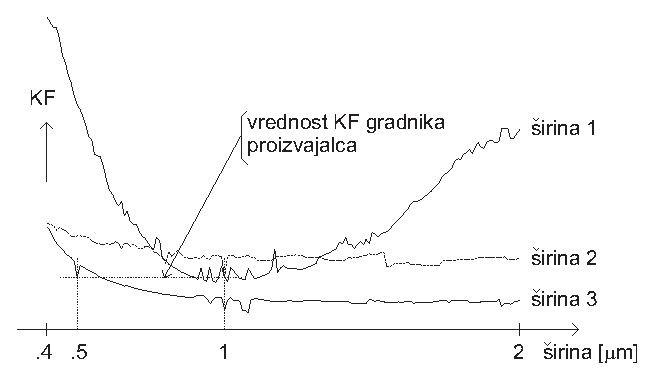
\includegraphics[width=8cm]{fig/cost_profile_slo}}
\caption{Preseki kriterijske funkcije po treh širinah kanalov}
\label{cost_profile}
\end{figure}

Na sliki \ref{cost_profile} je jasno viden numeričen šum, ki je posledica končnega časovnega koraka v tranzientni analizi. Z zmanjševanjem časovnega koraka postaja numeričen šum manjši. Vendar fino določanje končne rešitve z lokalno optimizacijsko metodo ne uspe, neglede na to kako majhen je  časovni korak. Zato je potrebno celoten optimizacijski tek izvesti z robustno globalno metodo. Za zagotovitev točnosti mora biti časovni korak kljub temu relativno majhen, kar pomeni dolge tranzientne analize in posledično dolge optimizacijske teke. En optimizacijski tek traja pet dni na osmih paralelnih procesorjih.

\section{Zaključek}
Osnovni digitalni gradniki podani v knjižnici proizvajalca predstavljajo nabor gradnikov, ki naj jih načrtovalec integriranih vezij na tranzistorskem nivoju ne bi spreminjal. Primer v članku pokaže znatno izoljšanje lastnosti osnovnega gradnika z uporabo optimizacijskega postopka na tranzistorskem nivoju. Doseženo je bilo do 77\% izboljšanje časovnih lastnosti gradnika brez povečanja porabe. Oziroma na drugi strani 20\% zmanjšanje porabe ob enakih časovnih lastnostih. Uporaba gradnikov prirejenih na specifične zahteve v vezju bi lahko vodila k hitrejšim digitalnim vezjem z nižjo porabo. Da bi predlagan postopek postal učinkovit, bi bilo potrebno optimizacijo na tranzistorskem nivoju vključiti v orodja za sintezo. Dolžina optimizacijskih tekov ostaja zaradi šumnosti poteka kriterijske funkcije glavna ovira. Ponovna preveritev optimiziranih gradnikov v sintezacijskem orodju zaradi nedostopnosti (plačljivosti) slednjih, kakor tudi zaradi nedostopnosti orodij za ekstrakcijo opisa gradnika iz tranzistorskega na višji nivo (proizvajalci integriranih vezij ekstrakcijskih orodij ne podajajo), ni bila narejena.

\section*{Zahvala}
Raziskavo je omogočilo Ministrstvo za visoko šolstvo, znanost in tehnologijo Republike Slovenije v okviru programa P2-0246 - Algoritmi in optimizacijski postopki v telekomunikacijah.

\begin{thebibliography}{10}
\bibitem{kaeslin} H.~Kaeslin, {\em Digital integrated circuit design: from VLSI architectures to CMOS fabrication}, \hskip 1em plus 0.5em minus 0.4em \relax Cambridge University Press, 2008.

\bibitem{hspice} {\em HSPICE\textsuperscript{\textregistered} simulation and analysis user guide}, \hskip 1em plus 0.5em minus 0.4em \relax Synopsys\textsuperscript{\textregistered}, 2005.

\bibitem{kunderth} K.S.~Kunderth, {\em The designer's guide to SPICE and Spectre}, \hskip 1em plus 0.5em minus 0.4em \relax Kluwer Academic Publishers, 1995.

\bibitem{virtuoso} {\em Virtuoso\textsuperscript{\textregistered} Spectre\textsuperscript{\textregistered} circuit simulator user guide}, \hskip 1em plus 0.5em minus 0.4em \relax Cadence Design Systems, Inc., 2008.

\bibitem{tuma} T.~Tuma, \'{A}.~B\H{u}rmen, {\em Circuit simulation with SPICE Opus, theory and practice}, \hskip 1em plus 0.5em minus 0.4em \relax Birkh\"{a}user, 2009.

\bibitem{thomas} D.E.~Thomas, P.R.~Moorby, {\em The Verilog hardware description language}, 5\textsuperscript{th}~ed. \hskip 1em plus 0.5em minus 0.4em \relax Kluwer Academic Publishers, 2003.

\bibitem{pedroni} V.A.~Pedroni, {\em Circuit design with VHDL}, \hskip 1em plus 0.5em minus 0.4em \relax Massachusetts Institute of Technology, 2004.

\bibitem{kurup} P.~Kurup, T.~Abbasi, {\em Logic synthesis using Synopsys\textsuperscript{\textregistered}}, 2\textsuperscript{nd}~ed. \hskip 1em plus 0.5em minus 0.4em \relax Kluwer Academic Publishers, 1997.

\bibitem{bhatnagar} H.~Bhatnagar, {\em Advanced ASIC chip synthesis using Synopsys\textsuperscript{\textregistered} Design Compiler\texttrademark Physical Compiler\texttrademark and PrimeTime\textsuperscript{\textregistered}}, 2\textsuperscript{nd}~ed. \hskip 1em plus 0.5em minus 0.4em \relax Kluwer Academic Publishers, 2002.

\bibitem{burmen1} \'{A}.~B\H{u}rmen et al., ``Automated robust design and optimization of integrated circuits by means of penalty functions,'' \hskip 1em plus 0.5em minus 0.4em \relax {\em AE\"{U}, International Journal of Electronics and Communications}, vol. 57, no. 1, pp. 47--56, 2003.

\bibitem{olensek} J.~Olen\v{s}ek, \'{A}.~B\H{u}rmen, J.~Puhan, T.~Tuma, ``DESA: a new hybrid global optimization method and its application to analog integrated circuit sizing,'' \hskip 1em plus 0.5em minus 0.4em \relax {\em Journal of Global Optimization}, vol. 44, no. 1, pp. 1--25, 2008.

\bibitem{hooke} R.~Hooke, T.~Jeeves, ``Direct search solutions of numerical and statistical problems,'' \hskip 1em plus 0.5em minus 0.4em \relax {\em Journal of the Association for Computing Machinery}, vol. 8, no. 2, pp. 212--229, 1961.

\bibitem{burmen2} \'{A}.~B\H{u}rmen, I.~Fajfar, T.~Tuma, ``Combined Simplex-Trust-Region optimization algorithm for automated IC design,'' \hskip 1em plus 0.5em minus 0.4em \relax {\em Proceedings of ECCTD07 European Conference on Circuit Theory and Design}, pp. 543--546, 2007.
\end{thebibliography}

\begin{IEEEbiographynophoto}{Janez Puhan} je leta 2000 doktoriral s področja elektrotehnike na Univerzi v Ljubljani. Je asistent na Fakulteti za elektrotehniko. Njegovo področje raziskovanja obsega modeliranje, simulacijo in optimizacijske postopke pri računalniškem načrtovanju vezij.
\end{IEEEbiographynophoto}

\begin{IEEEbiographynophoto}{Iztok Fajfar} je diplomiral (1991), magistriral (1994) in doktoriral (1997) s področja elektrotehnike na Fakulteti za elektrotehniko Univerze v Ljubljani. V letu 1991 je bil raziskovalec na Inštitutu Jožef štefan v Ljubljani, nakar je konec leta zasedel raziskovalno mesto na Fakulteti za elektrotehniko Univerze v Ljubljani. 
Trenutno na fakulteti zaseda mesto izrednega profesorja. Poučuje več uvodnih in nadaljevalnih predmetov s področja računalniškega programiranja. Pri razvoju programske opreme je sodeloval v več industrijskih projektih s podjetji Adacta in ICE Telecom. Njegovo področje raziskovanja vključuje načrtovanje in optimizacijo elektronskih vezij.
\end{IEEEbiographynophoto}

\begin{IEEEbiographynophoto}{Tadej Tuma} je diplomiral (1988), magistriral (1991) in doktoriral (1995) na Fakulteti za elektrotehniko Univerze v Ljubljani. Na isti fakulteti je redni profesor, kjer poučuje štiri dodiplomske in tri podiplomske predmete. Njegovi raziskovalni interesi so predvsem na področju računalniške analize in načrtovanja vezij.
\end{IEEEbiographynophoto}

\begin{IEEEbiographynophoto}{\'{A}rp\'{a}d B\H{u}rmen} se je rodil leta 1976 v Murski Soboti. Leta 2003 je na Univerzi v Ljubljani doktoriral s področja elektrotehnike. Od leta 2005 dalje je docent na fakulteti za elektrotehniko. Njegovo raziskovalno področje vključuje zvezno in dogodkovno simulacijo vezij in sistemov, optimizacijske metode, njihovo konvergenco in uporabo, ter algoritme za vzporedno in porazdeljeno računanje. Je eden vodilnih razvijalcev simulatorja vezij SPICE OPUS. Objavil je preko 20 člankov v recenziranih revijah.
\end{IEEEbiographynophoto}

\vfill

\label{finish}

% that's all folks
\end{document}


